\documentclass[c]{beamer}

%\usepackage[sorting=none]{biblatex}

\usepackage{url}
\usetheme{CambridgeUS}
\usecolortheme{dolphin}
\setbeamercolor{footline}{fg=white, bg=black}
\usepackage[backend=bibtex, sorting=none, maxbibnames=5]{biblatex}
\renewcommand*{\bibfont}{\tiny}
\setbeamertemplate{bibliography item}{\insertbiblabel}
\renewcommand{\footnotesize}{\tiny}
\usefonttheme{professionalfonts}
\bibliography{seminar}
%\bibliographystyle{unsrt}
%%%%%    set the bullet style to rectangles   %%%%%
\useinnertheme{rectangles}

%%% change default style of beamer bibliography %%%
\setbeamertemplate{bibliography item}{\insertbiblabel}

%%%%%%%%   remove bottom navigation bar   %%%%%%%%%
\beamertemplatenavigationsymbolsempty
\usepackage{ragged2e}       %justification
\usepackage{graphicx} 		% Allows including images
\usepackage{fixltx2e} 		% need to use the \textsubscript{} command
\usepackage{algorithmic} 	% need to write some algorithms
\usepackage{amsmath}		% need to write some equations

\title[My Seminar Title in Footer]{\textbf{My Seminar Title on Title Page}}
%\titlegraphic{
\includegraphics[width=2cm,height=1.5cm]{logo.jpg}}
\author[Name of Student (Reg No)] % (optional, for multiple authors)
{\large
\vspace{3mm}		
Name of Student (Reg No)	\\	
\vspace{3mm}
S\textsubscript{7} B.Tech CSD \\ 
\vspace{3mm}
\emph{Guided by:}
Name and Designation of Guide \\[12pt]
\makebox[\textwidth]{

\includegraphics[width=2cm,height=1.5cm]{logo.jpg}} \\[6pt]
Department of Computer Science and Engineering\\
Government Engineering College,Kozhikode \\
}
\date[]{\today}
\subject{Seminar Presentation}

%%%%%%%%%%%%%%%%%%%%%%%%%%%%%%%%%%%%%%%%%%%%%%%%%%%%%%%%%%%%%%%%%%%%%%%%
%% Uncomment this to include a table of contents before every section %%
%%%%%%%%%%%%%%%%%%%%%%%%%%%%%%%%%%%%%%%%%%%%%%%%%%%%%%%%%%%%%%%%%%%%%%%%

%\AtBeginSection[]
%{
%	\begin{frame}[plain]{Outline}
%	\tableofcontents[currentsection]
%	\end{frame}
%}

\begin{document}
%%%%%%%%%%%%%%%%%%%%%%%%%%%%%%%%%%%%%%
\begin{frame}[plain]
  \titlepage
\end{frame}

\begin{frame}
\frametitle{\textbf{Outline:}}
\tableofcontents
\end{frame}



%%%%%%%%%%%% Introduction %%%%%%%%%%%%
\section{INTRODUCTION}
	
\begin{frame}
\frametitle{Introduction}
    \begin{itemize}
    \justifying
        \item \textbf{MACHINE LEARNING} 
        \item ------------------------------------------------------------------------------\\
         \item -----------------------------
    \end{itemize}			
\end{frame}

\begin{frame} [c]
    \frametitle{Introduction}
    \begin{itemize}
    \justifying
         \item \textbf{FEATURE EXTRACTION} 
         \item --------------------------
         \item ------------------------------
    \end{itemize}
\end{frame}
%%%%%%%%%%%% Background %%%%%%%%%%%%%%

     
	
	

 %%%%%%%%%%%% OBJECTIVES %%%%%%%%%%%%

\section{OBJECTIVES}	
\begin{frame} [c]
    \frametitle{Objectives Of Seminar}
    \begin{itemize}
    \justifying
      \item \textbf{---} 
        \item ------------------------------------------------------------------------------
         \item -----------------------------
    \end{itemize}			
\end{frame}
%%%%%%%%%%%%%%%%%%%%%%%%%%%%%%%%%%%%%
\section{MOTIVATION}               
\begin{frame} [c]
\frametitle{MOTIVATION}
\begin{itemize}
    \justifying
         \item Point 1
         \item Point 2
         \item Point 3....
    \end{itemize}
    %\begin{figure}
    %    \centering
       % \includegraphics[width=7cm]{images/overview.png}
      %  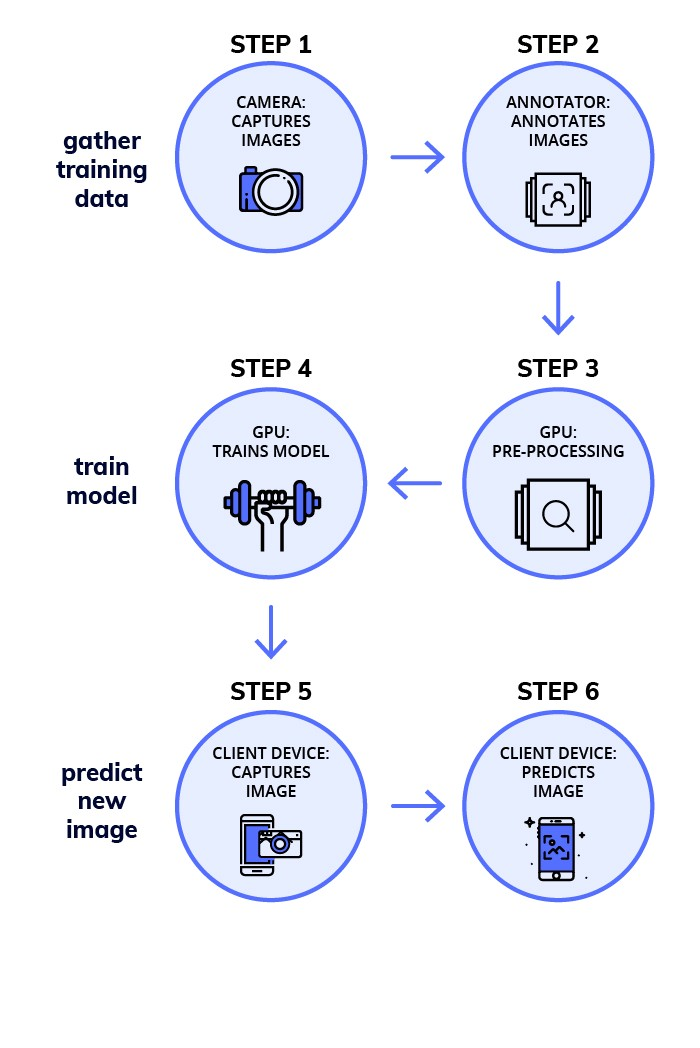
\includegraphics[scale=.18]{ten.jpeg}
      %  \caption{Workflow of Object Detection}
      %  \label{Workflow of Object Detection}
   % \end{figure}
   
\end{frame}
	
	
\section{LITERATURE SURVEY/RELATED WORKS}
\begin{frame} [c]
    \frametitle{Related Work(s)-1-Sample}
    \begin{itemize}
    \justifying
          \item Martinus \footfullcite{AssistingTourism} developed an Mobile Application as a “Virtual game ranger”, for identifying the wild animals in less known game reserves of Africa. 

        \item Researchers at PlantVillage and the International Institute of Tropical Agriculture (IITA) \footfullcite{Plant}has used ML and TensorFlow to help farmers detect diseases in Cassava plants.
       \end{itemize} 
      
\end{frame}
\begin{frame} [c]
    \frametitle{Related Work-2-Sample}
    \begin{itemize}
    \justifying
          \item Martinus\footfullcite{AssistingTourism} developed an Mobile Application as a “Virtual game ranger”, for identifying the wild animals in less known game reserves of Africa.

        \item Researchers at PlantVillage and the International Institute of Tropical Agriculture (IITA) \footfullcite{Plant} has used ML and TensorFlow to help farmers detect diseases in Cassava plants.
       \end{itemize} 
      
\end{frame}
\begin{frame} [c]
    \frametitle{Related Work-3-Sample}
    \begin{itemize}
    \justifying
          \item Martinus\footfullcite{AssistingTourism} developed an Mobile Application as a “Virtual game ranger”, for identifying the wild animals in less known game reserves of Africa.

        \item Researchers at PlantVillage and the International Institute of Tropical Agriculture (IITA) \footfullcite{Plant}has used ML and TensorFlow to help farmers detect diseases in Cassava plants.
       \end{itemize} 
      
\end{frame}
\section{METHODOLOGY/ALGORITHMS}

    \begin{frame} [c]
    \frametitle{Method/Alg 1----Specify the name of  methods/algorithms discussed in paper 1}
    \begin{itemize}
    \justifying
      \item \textbf{Name-Method 1}
      \item Point 1
      \item Point 2
      \item Point 3....
    \end{itemize}
   % \begin{figure}
      %  \centering
       % \includegraphics[width=7cm]{images/overview.png}
     %   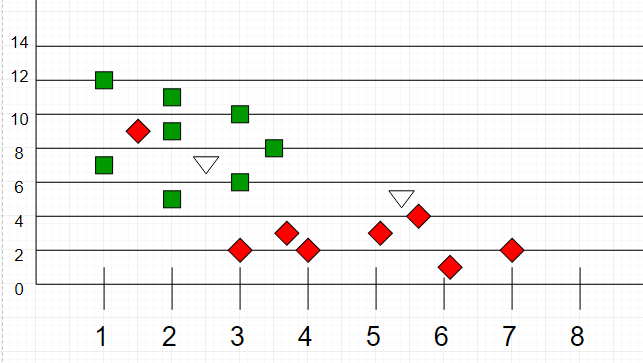
\includegraphics[scale=.46]{graph2-2.png}
      %  \caption{K-nearest neighbour}
     %   \label{K-nearest neighbour}
    %\end{figure}
        \end{frame}
        
\begin{frame} [c]
\frametitle{Method/Alg 2----Specify the name of  methods/algorithms discussed in paper 2}
    \begin{itemize}
    \justifying
        \item \textbf{Name-Method 2} 
    
   % \begin{figure}
     %   \centering
       % \includegraphics[width=7cm]{images/overview.png}
     %   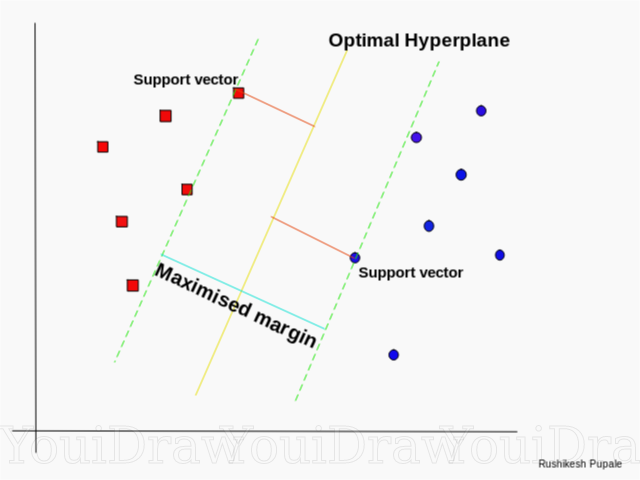
\includegraphics[scale=.32]{SVM.png}
     %   \caption{Support Vector Machine (SVM)}
     %   \label{Support Vector Machine (SVM)}
   % \end{figure}
   \item Point 1
   \item Point 2....
   \end{itemize}
\end{frame}
       
\begin{frame} [c]
\frametitle{Method/Alg 2----Specify the name of  methods/algorithms discussed in paper 2}
\begin{itemize}  
\justifying       
    \item \textbf{Method 2} 
\item Point 1
\item Point 2
\item Point 3 .....
\end{itemize}
%\begin{figure}
 %   \centering
   % \includegraphics[width=7cm]{images/overview.png}
 %   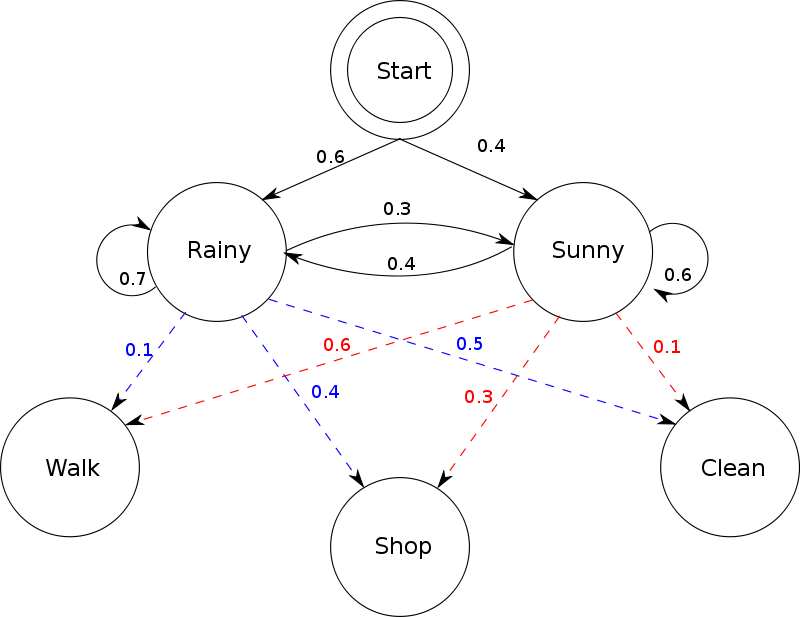
\includegraphics[scale=.25]{hmm.png}
 %   \caption{Hidden Markov Model (HMM)}
  %  \label{Hidden Markov Model (HMM)}
% \end{figure}
\end{frame}

\begin{frame}[c]
\frametitle{Method/Alg 3----Specify the name of  methods/algorithms discussed in paper 3}
    \begin{itemize}  
    \justifying       
        \item  \textbf{Method 3} 
        \item .......
        \item .......
        \item......
    \end{itemize}
    %\begin{figure}
     %   \centering
       % \includegraphics[width=7cm]{images/overview.png}
     %   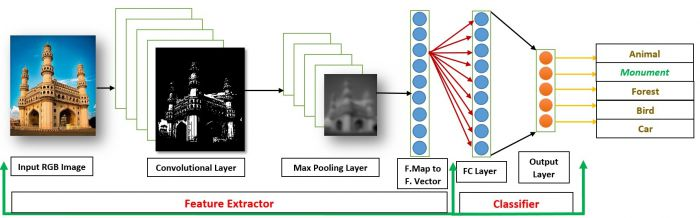
\includegraphics[scale=.5]{cnn.jpg}
      %  \caption{Convolutional Neural Network (CNN)}
      %  \label{Convolutional Neural Network (CNN)}
    % \end{figure}
\end{frame}

\section{OUTCOME OF THE SURVEY}               
\begin{frame} [c]
\frametitle{OUTCOME OF THE SURVEY}
\begin{itemize}  
\justifying       
    \item Include a table that shows the Methods, Merits, and Demerits of each Category

\end{itemize}

\begin{figure}
    \centering
    % \includegraphics[width=7cm]{images/overview.png}
    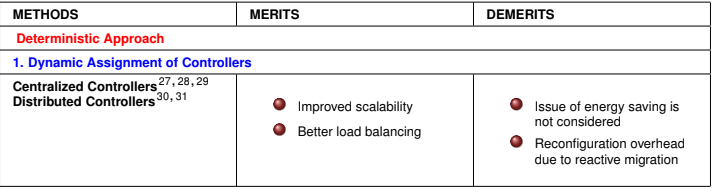
\includegraphics[scale=.5]{outcome.png}
    \caption{Outcome of the Literature....Dynamic Assignment of Controllers}
    \label{Outcome of the Literature....Deterministic Approach}
\end{figure}
\end{frame} 

\section{CONCLUSION}
\begin{frame} [c]
    \frametitle{CONCLUSION}
    \begin{itemize}
    \justifying
         \item Point 1
         \item Point 2
         \item Point 3....
    \end{itemize}
\end{frame}

\section{Approval by Guide}
\begin{frame} [c]
    \frametitle{Approval}
    \begin{itemize}
    
         \item Screenshot of Guide approval of Seminar Slide
         
    \end{itemize}
\end{frame}
%\section{REFERENCES}
%\section*{Bibliography}
%%%%%%%%%% Bibliography %%%%%%%%%%%%
	
\section{REFERENCES}
\begin{frame}[allowframebreaks]{REFERENCES}
\tiny
\nocite{*}
\printbibliography
\end{frame}
	
%	\begin{frame}[c]
%	
\includegraphics[scale=.7]{thnk.PNG}
%	\end{frame}
	
\end{document}
